\documentclass[pdf, aspectratio=169]{beamer}
\usepackage[]{hyperref, graphicx, siunitx, lmodern, tikz, booktabs, physics}
\usepackage{pgfplots, pgfplotstable}
\usepackage[mode=buildnew]{standalone}
\usepackage{pdfpc-commands}
\usepackage{intro-commands}

\usetheme{Astro}
\graphicspath{ {../Images/} }

\sisetup{per-mode=symbol}
\usetikzlibrary{calc, patterns, decorations.markings, decorations.pathmorphing, shapes}
\DeclareSIUnit\parsec{pc}

%Preamble
\title{Puffing up the Universe}
\author{Jed Rembold}
\date{November 30, 2018}

\begin{document}
\renewcommand{\theenumi}{\Alph{enumi}}

\begin{frame}{Announcements}
	\begin{itemize}
		\item Webwork due on Monday
		\item I'll have study materials for the final posted early next week.
		\item Physics Tea today at 3pm!
		\item Physics Talks by Seniors all afternoon, starting from 2 until 5
			\begin{itemize}
				\item Catch me afterwards if you have questions or need help on anything!
			\end{itemize}
		\item Blood Drive today! Donate your precious life-essence!
		\item Polling: \nolinkurl{rembold-class.ddns.net}
	\end{itemize}
\end{frame}

\begin{frame}{Spiral Galaxies}
  \begin{itemize}
	\item Many of the characteristics of the Milky Way
	  \begin{itemize}
		\item Spiral disk, bulge, halo, etc
	  \end{itemize}
	\item Can come in normal or barred varieties
  \end{itemize}
  \begin{center}
	\begin{tikzpicture}
	  \node<1-> at (3,1) {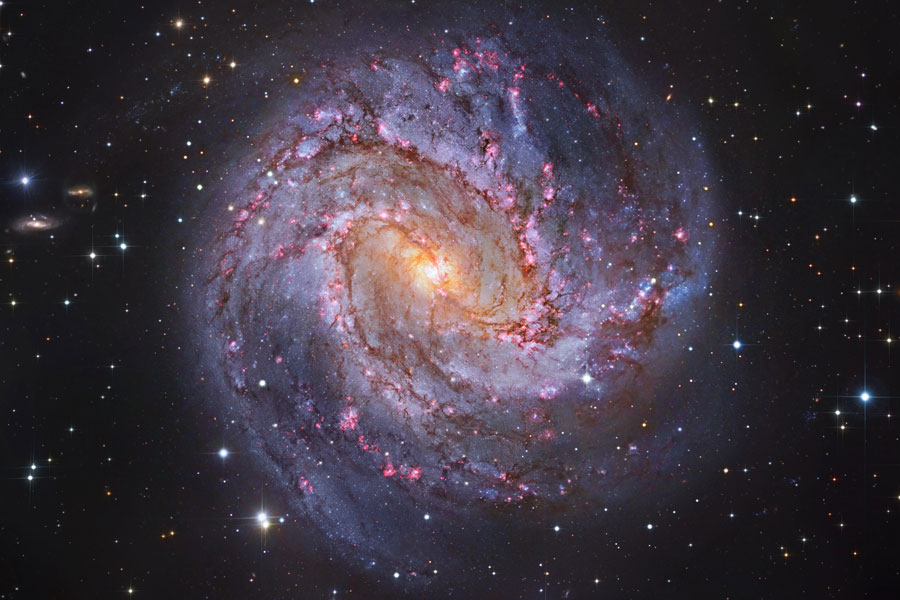
\includegraphics[width=5cm]{ch16_spiral3.jpg}};
	  \node<2-> at (0,0) {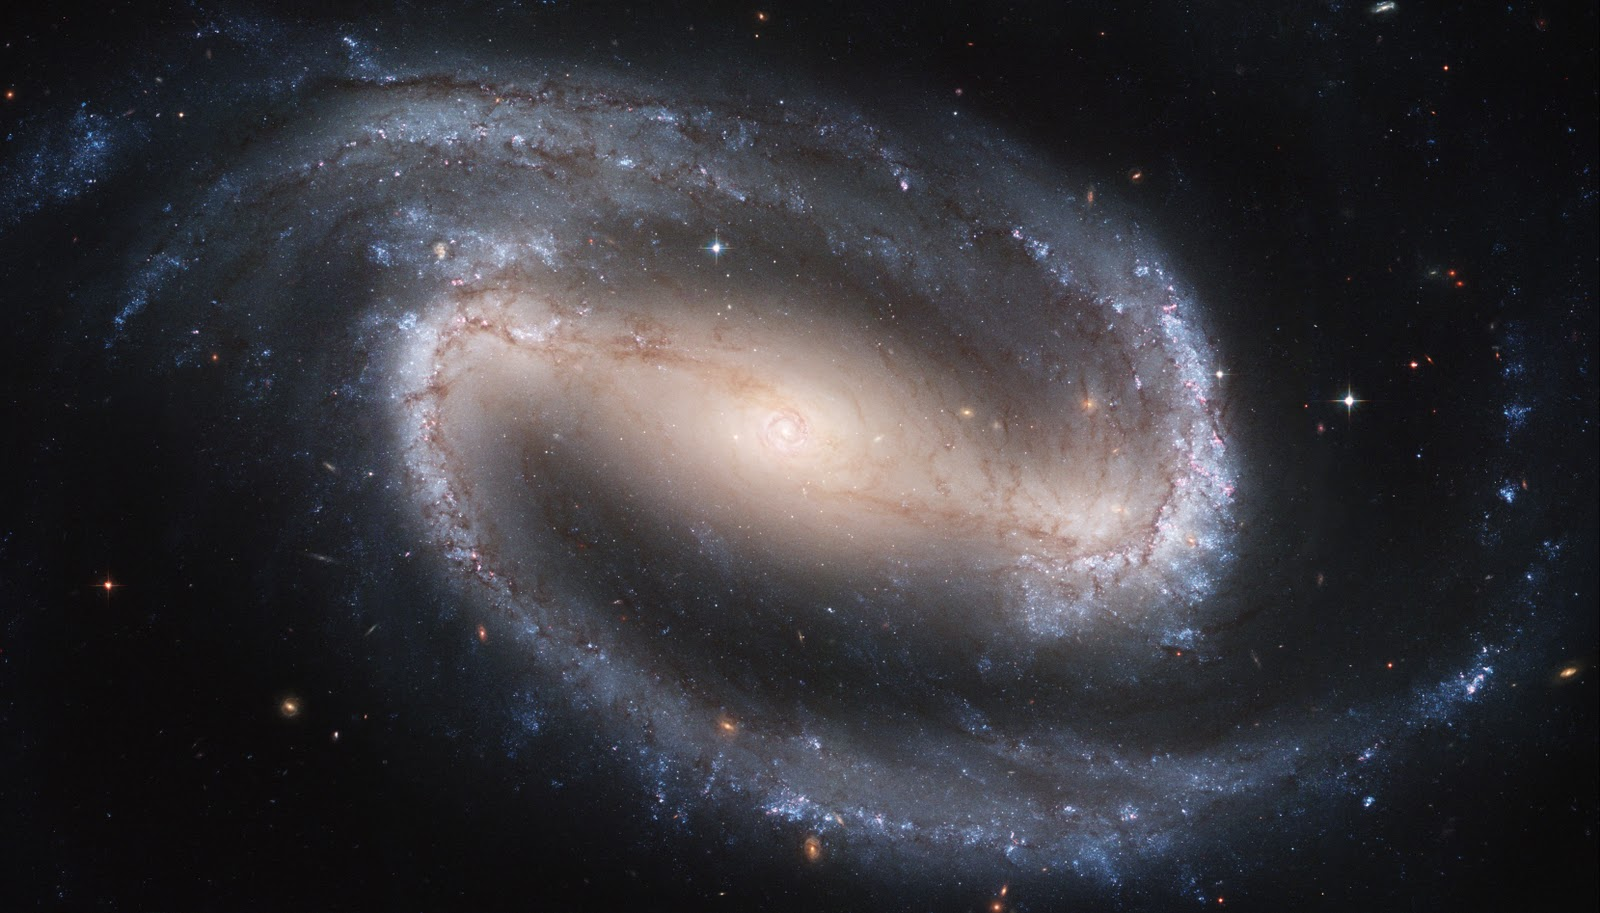
\includegraphics[width=5cm]{ch16_spiral2.jpg}};
	  \node<3-> at (-3,-1) {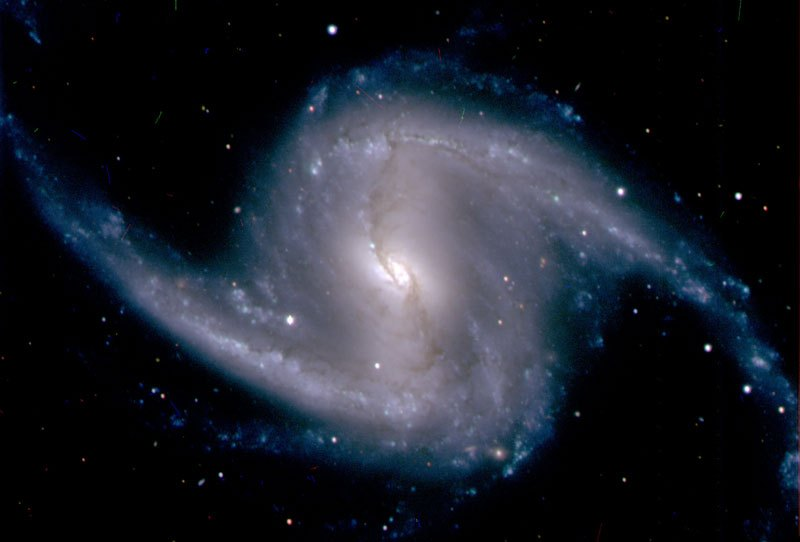
\includegraphics[width=5cm]{ch16_spiral4.jpg}};
	\end{tikzpicture}
  \end{center}
\end{frame}

\begin{frame}{Elliptical Galaxies}
  \begin{columns}
	\column{.5\textwidth}
	\begin{center}
	  \vspace{-6mm}
	  \begin{tikzpicture}
		\node at (0,0) {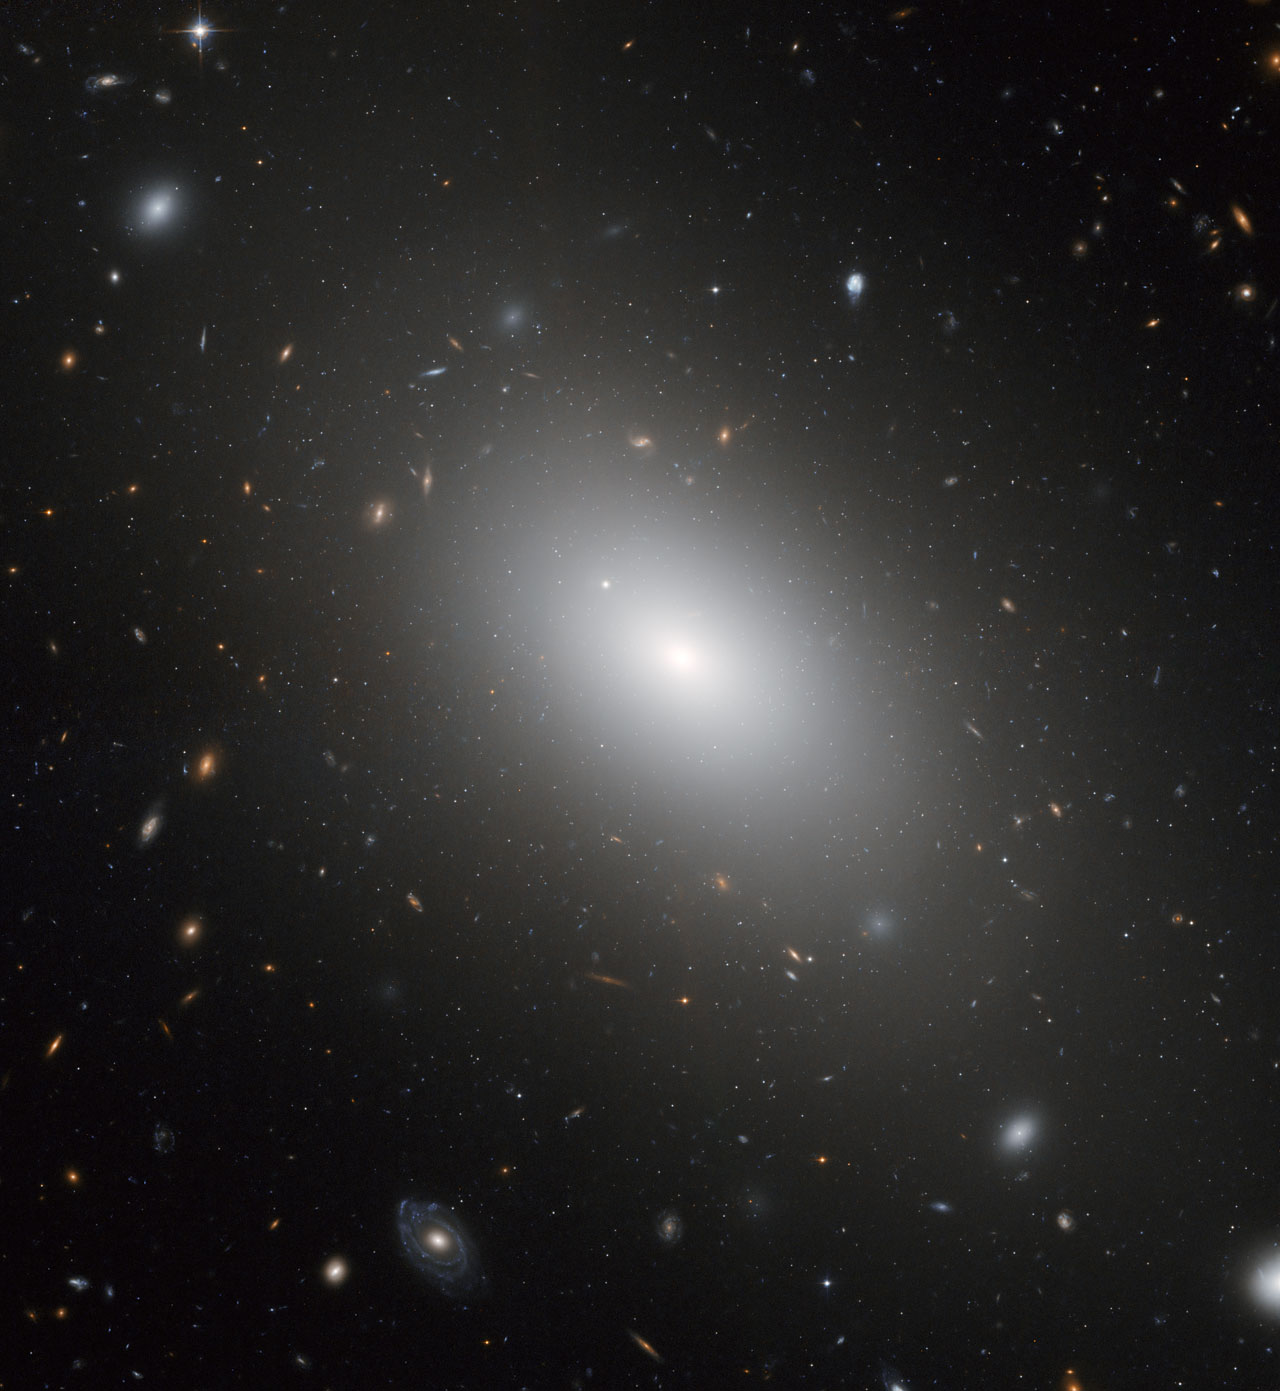
\includegraphics[width=4cm]{ch16_elliptical2.jpg}};
		\node at (2,-3) {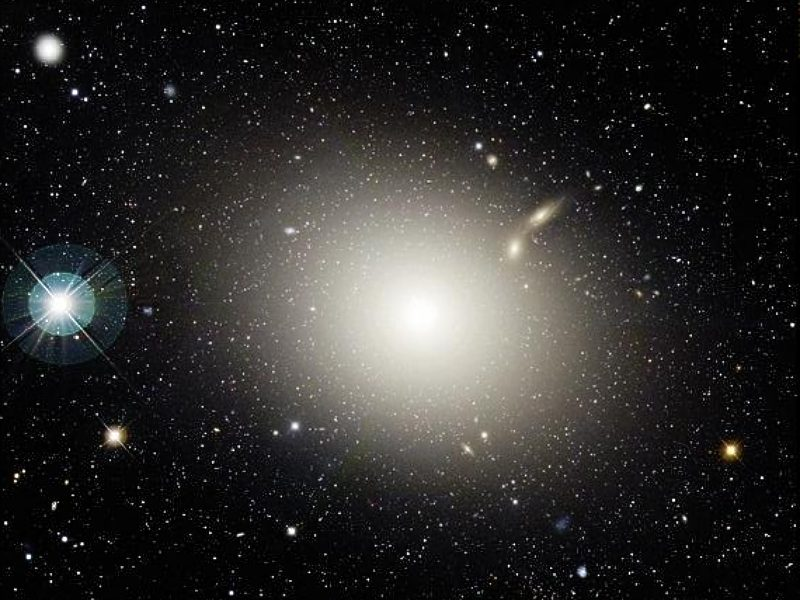
\includegraphics[width=5cm]{ch16_elliptical3.jpg}};
	  \end{tikzpicture}
	\end{center}
	\column{.5\textwidth}
	\begin{itemize}
	  \item Differ from spirals is important ways:
		\begin{itemize}
		  \item Have no disk
		  \item Rotate more slowly
		  \item Contain very little gas or dust
		  \item Contain mainly old stars
		  \item Huge range of sizes
			\begin{itemize}
			  \item 0.0001--100 times the Milky Way
			\end{itemize}
		\end{itemize}
	\end{itemize}
  \end{columns}
\end{frame}

\begin{frame}{Irregular Galaxies}
  \begin{itemize}
	\item The misfits
	\item Often times harbor very active star forming regions
	\item Can sometimes be the result of galaxy collisions
  \end{itemize}
  \begin{center}
	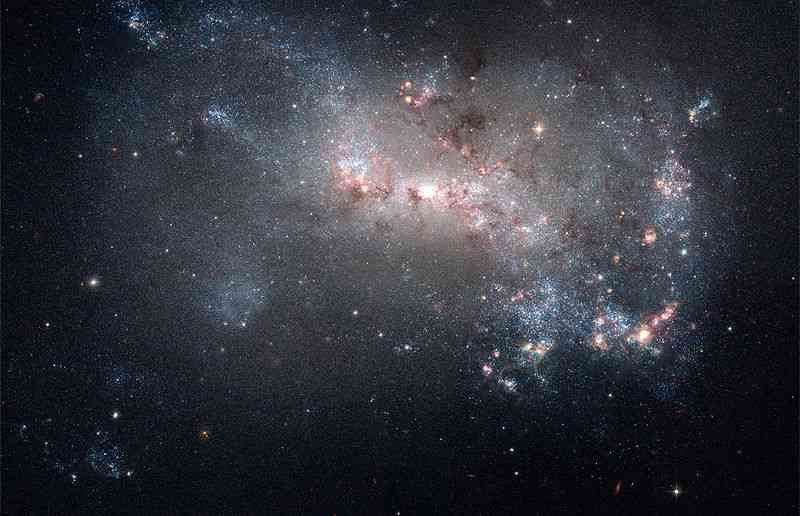
\includegraphics[width=.45\textwidth]{ch16_irregular2.jpg}
	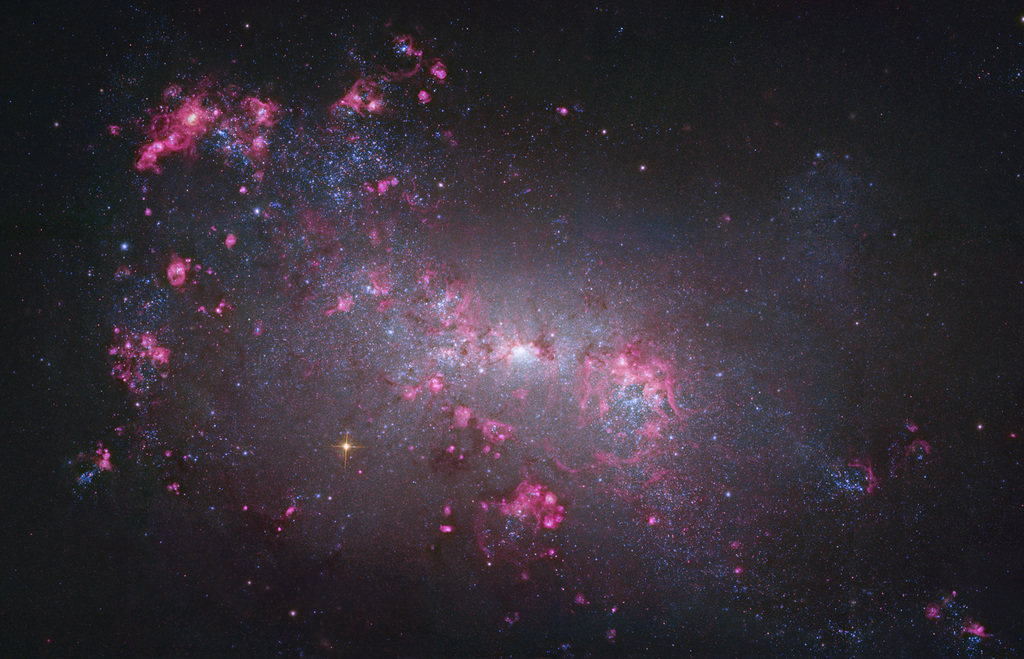
\includegraphics[width=.45\textwidth]{ch16_irregular3.jpg}
  \end{center}
\end{frame}

\begin{frame}{Hubble's Fork}
  \begin{center}
	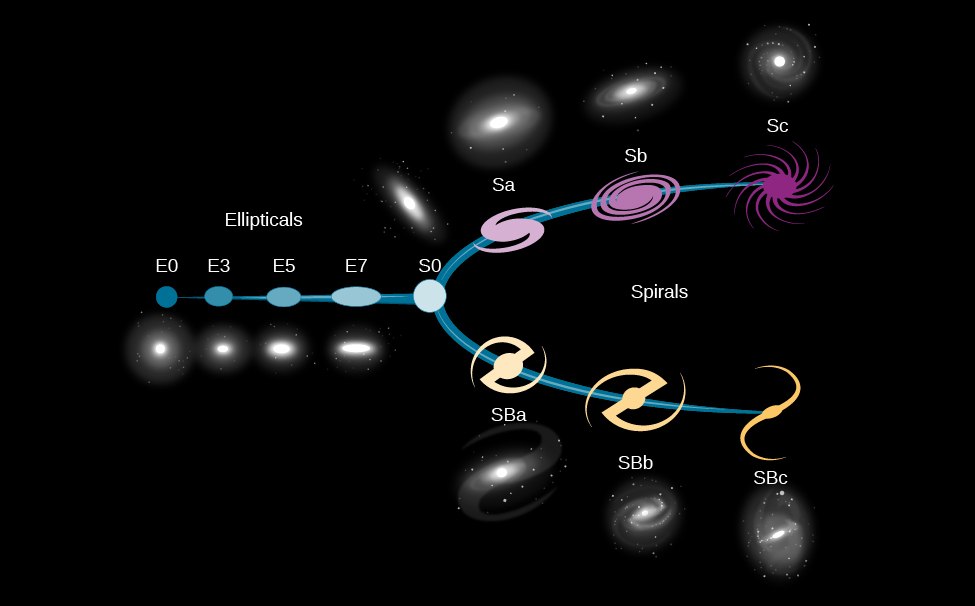
\includegraphics[width=.8\textwidth]{ch26_hubble_fork.jpg}
  \end{center}
\end{frame}

\begin{frame}{Back to the Darkness}
	The Milky Way is not unique with its rotation curve!
  \begin{center}
	\begin{tikzpicture}
	  \begin{axis}[
		  width=\textwidth,
		  height=7cm,
		  xlabel=Distance from Center (in 1000 lyrs),
		  ylabel=Orbital Speed (km/s),
		  legend pos = south east,
		  legend style={fill=none, draw=none},
		]
		\addplot[yellow!70!orange, smooth, very thick] table[x index=0, y index=1] {../Data/UGC2885.csv};
		\addplot[smooth, very thick, green!50!cyan] table[x index=0, y index=1] {../Data/NGC7541.csv};
		\addplot[smooth, very thick, red!70!violet] table[x index=0, y index=1] {../Data/NGC801.csv};
		\addplot[smooth, very thick, cyan] table[x index=0, y index=1] {../Data/NGC2998.csv};
		\legend{UGC 2885, NGC 7541, NGC 801, NGC 2998}
	  \end{axis}
	\end{tikzpicture}
  \end{center}
\end{frame}

\begin{frame}{Macho Man!}
  \begin{columns}
	\column{.4\textwidth}
	\begin{itemize}
	  \item How else could we get invisible mass?
	  \item Could the halo be filled with faint, dead stars?
		\begin{itemize}
		  \item \alert{Ma}ssive \alert{C}ompact \alert{H}alo \alert{O}bjects
		  \item Brown Dwarfs
		  \item Neutron Stars
		  \item Black Holes
		\end{itemize}
	  \item How does one find an invisible object?
	\end{itemize}
	\column{.6\textwidth}
	\begin{center}
	  \includegraphics[width=\textwidth]{ch16_brown_dwarfs.jpg}
	\end{center}
  \end{columns}
\end{frame}

\begin{frame}{Gravitational (Micro)lensing}
  \begin{itemize}
	\item We look for their mass's effect on nearby light
	\item Find that MACHOs account for 20\% of the missing halo mass at most
	\item So dark matter definitely still on the table\ldots
  \end{itemize}
  \begin{center}
	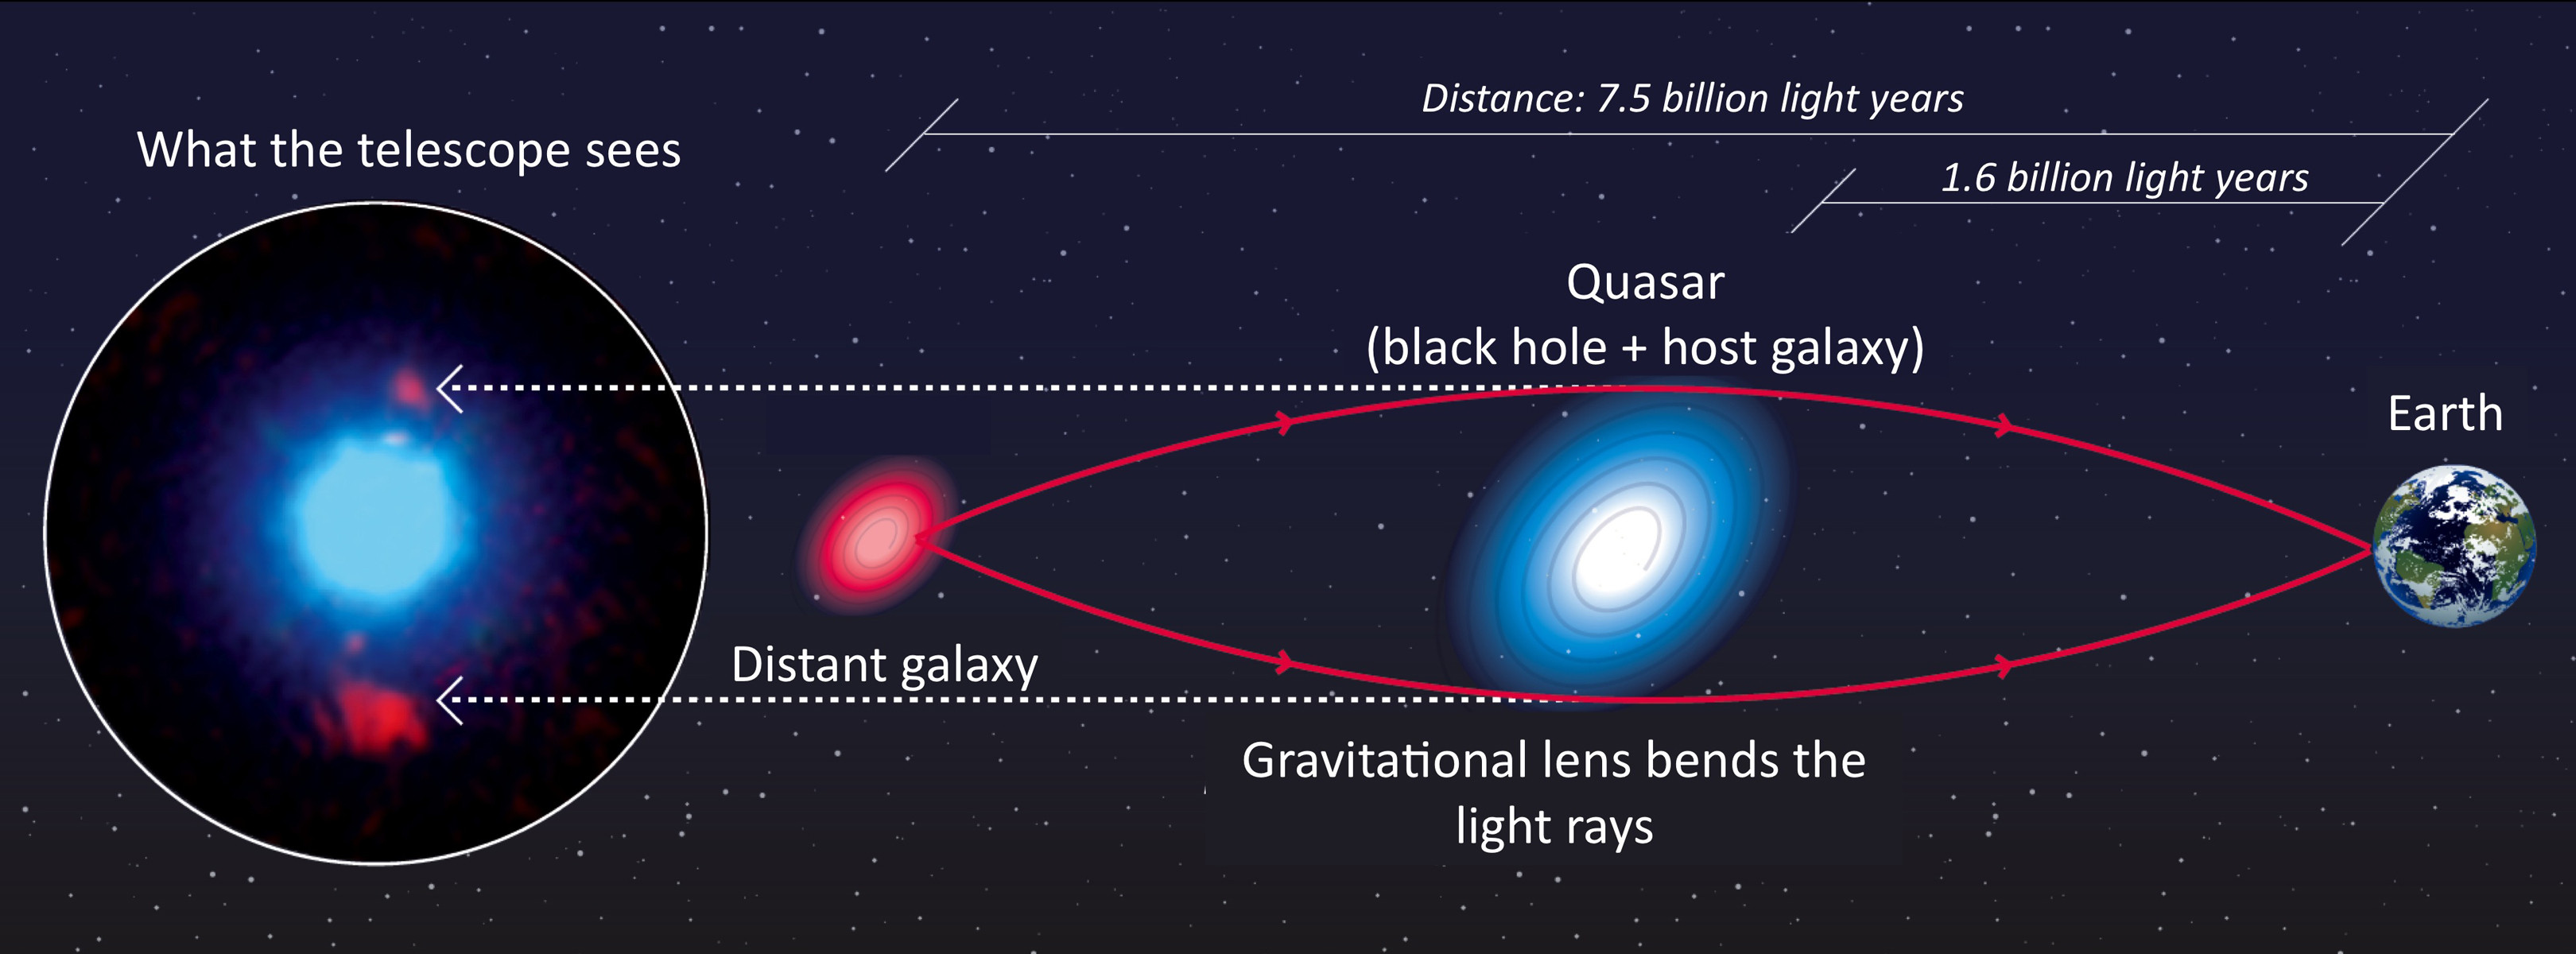
\includegraphics[width=\textwidth]{ch16_lensing}
  \end{center}
\end{frame}
\begin{frame}{Social Galaxies}
  \begin{columns}
	\column{.4\textwidth}
	\begin{itemize}
	  \item Galaxies tend to group up
		\begin{itemize}
		  \item Compared to their size, distances between galaxies much smaller than distances between stars
		\end{itemize}
	  \item Milky Way is part of the aptly named Local Group
	\end{itemize}
	\column{.6\textwidth}
	\begin{center}
	  \includegraphics[width=.8\textwidth]{ch16_LocalGroup.png}
	\end{center}
  \end{columns}
\end{frame}

\begin{frame}{Clusters also want friends}
  \begin{itemize}
	\item Clusters and Groups also tend to group up, forming \alert{superclusters}!
  \end{itemize}
  \begin{center}
	\includegraphics[width=.7\textwidth]{ch16_Virgocluster.jpg}
  \end{center}
\end{frame}

\fullFrameImage{ch16_supercluster.png}

\begin{frame}{Understanding Check}
  Which of the following is NOT one of the ways that elliptical galaxies differ from spiral galaxies?
  \begin{enumerate}
	\item They have no galactic disk
	\item \alert<2>{They have mainly younger type stars}
	\item They rotated more slowly
	\item They contain little gas or dust
  \end{enumerate}
\end{frame}

\begin{frame}{The Distance Ladder}
  \begin{center}
	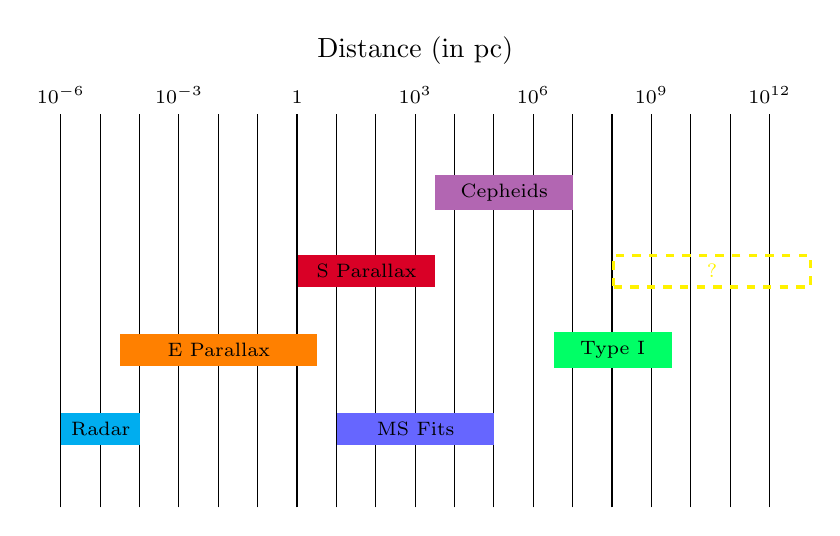
\begin{tikzpicture}
	  \foreach \x in {-1.0,-.5,...,8}{
		\draw (\x,0) --+(0,5);
	  }
	  \node[above] at (3.5,5.5) {Distance (in pc)};
	  \begin{scope}[font=\scriptsize]
		\node[above] at (-1.0,5) {$10^{-6}$};
		\node[above] at (0.5,5) {$10^{-3}$};
		\node[above] at (2.0,5) {$1$};
		\node[above] at (3.5,5) {$10^3$};
		\node[above] at (5.0,5) {$10^6$};
		\node[above] at (6.5,5) {$10^9$};
		\node[above] at (8.0,5) {$10^{12}$};
		\node[black,fill=cyan, anchor=west, minimum width=1cm] at (-1,1) {Radar};
		\node[black,fill=orange, anchor=west, minimum width=2.5cm] at (-.25,2) {E Parallax};
		\node[black,fill=red!70!violet, anchor=west, minimum width=1.75cm] at (2.0,3) {S Parallax};
		\node[black,fill=violet!60, anchor=west, minimum width=1.75cm] at (3.75,4) {Cepheids};
		\node[black,fill=blue!60, anchor=west, minimum width=2.0cm] at (2.5,1) {MS Fits};
		\node[black,fill=green!60!cyan, anchor=west, minimum width=1.5cm] at (5.25,2) {Type I};
		\node[draw, very thick, dashed, yellow, anchor=west, minimum width=2.5cm] at (6,3) {?};
	  \end{scope}

	\end{tikzpicture}
  \end{center}
\end{frame}

\begin{frame}{A Red Tale}
  \begin{itemize}
	\item Vesto Melvin Slipher - 1912
	  \begin{itemize}
		\item While observing spiral galaxies found that they \alert{all} seemed to be redshifted by various amount
		\item This would imply that all the distant galaxies were moving away from us!
	  \end{itemize}
	\item Edwin Hubble - 1929
	  \begin{itemize}
		\item Used Type Ia supernova to estimate distances to distant galaxies
		\item Found that the more distant galaxies were more redshifted
	  \end{itemize}
  \end{itemize}
  \begin{alertblock}<2>{The Hubble Relation}
	The more distant an object is, the faster it is moving away from us!
  \end{alertblock}
\end{frame}

\begin{frame}{Hubble's Law}
  \begin{center}
	\begin{tikzpicture}
	  \begin{axis}[
		  width=.9\textwidth,
		  height=7cm,
		  scaled ticks = false,
		  xlabel = Distance (\si{\mega\parsec}),
		  ylabel = Velocity (\si{\kilo\meter\per\second}),
		  ylabel near ticks,
		]
		\addplot[only marks] table[x index=0, y index=1] {../Data/Hubble.csv};
		\only<2>{\addplot[red,ultra thick] table[y={create col/linear regression={y=1}}] {../Data/Hubble.csv};}
		\node<2>[red] at (axis cs:350,15000) {$v=Hd$};
	  \end{axis}
	\end{tikzpicture}
  \end{center}
\end{frame}

\begin{frame}{The Hubble Constant}
  \begin{columns}
	\column{.5\textwidth}
	\begin{itemize}
	  \item Has varied greatly throughout its lifetime
		\begin{itemize}
		  \item Initially around 600 and took about 40 years to hone down to it near its current value
		\end{itemize}
	  \item Still empirically (experimentally) determined
	  \item Current estimates range between 65--79
	  \item Best value at the moment thought to be about
		\[H = \SI{72}{\kilo\meter\per\second\per\mega\parsec}\]
	\end{itemize}
	\column{.5\textwidth}
	\begin{center}
	  \begin{tikzpicture}
		\begin{axis}[
			width=\textwidth,
			height=7cm,
			/pgf/number format/.cd, use comma, 1000 sep={},
			ylabel=H,
			xticklabel style = {rotate=90},
		  ]
		  \addplot[black, fill=orange, only marks] table[x index=0, y index=1] {../Data/HubbleAge.csv};
		\end{axis}
	  \end{tikzpicture}
	\end{center}
  \end{columns}
\end{frame}

\begin{frame}{The Ultimate Range Finder}
  \begin{itemize}
	\item At extreme distances, Hubble's Law itself can be used to estimate the distance to a galaxy!
  \end{itemize}
  \begin{center}
	\vspace{-5mm}
	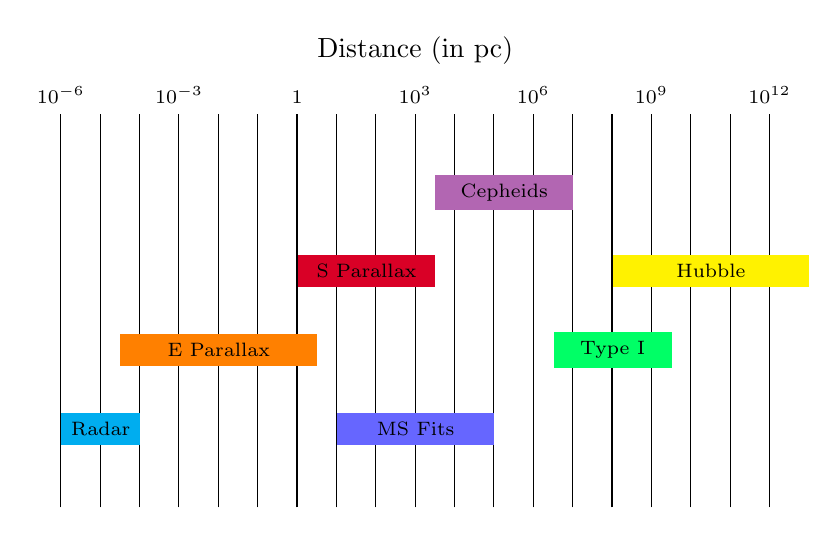
\begin{tikzpicture}
	  \foreach \x in {-1.0,-.5,...,8}{
		\draw (\x,0) --+(0,5);
	  }
	  \node[above] at (3.5,5.5) {Distance (in pc)};
	  \begin{scope}[font=\scriptsize]
		\node[above] at (-1.0,5) {$10^{-6}$};
		\node[above] at (0.5,5) {$10^{-3}$};
		\node[above] at (2.0,5) {$1$};
		\node[above] at (3.5,5) {$10^3$};
		\node[above] at (5.0,5) {$10^6$};
		\node[above] at (6.5,5) {$10^9$};
		\node[above] at (8.0,5) {$10^{12}$};
		\node[black,fill=cyan, anchor=west, minimum width=1cm] at (-1,1) {Radar};
		\node[black,fill=orange, anchor=west, minimum width=2.5cm] at (-.25,2) {E Parallax};
		\node[black,fill=red!70!violet, anchor=west, minimum width=1.75cm] at (2.0,3) {S Parallax};
		\node[black,fill=violet!60, anchor=west, minimum width=1.75cm] at (3.75,4) {Cepheids};
		\node[black,fill=blue!60, anchor=west, minimum width=2.0cm] at (2.5,1) {MS Fits};
		\node[black,fill=green!60!cyan, anchor=west, minimum width=1.5cm] at (5.25,2) {Type I};
		\node[black, fill=yellow, anchor=west, minimum width=2.5cm] at (6,3) {Hubble};
	  \end{scope}

	\end{tikzpicture}
  \end{center}
\end{frame}

%\begin{frame}{Understanding Check!}
  %A distance galaxy is measured to be moving away from us at \SI{1000}{\kilo\meter\per\second}. How far is it from us?
  %\begin{enumerate}
	%\item \SI{72000}{\parsec}
	%\item \alert<2>{\SI{14}{\mega\parsec}}
	%\item \SI{1000}{\mega\parsec}
	%\item \SI{72000}{\mega\parsec}
  %\end{enumerate}
%\end{frame}

\begin{frame}{Puffing Up}
  \begin{itemize}
	\item So all galaxies are moving away from us, but surely we aren't in the center?
	  \begin{itemize}
		\item \textcolor{Red}{Nope!}
		\item But then again, neither is anyone else!
	  \end{itemize}
	\item The Cosmological Principle:
	  \begin{itemize}
		\item At a given cosmic time, the universe looks basically the same to all observers.
	  \end{itemize}
	\item Everyone sees everything moving away because the entire universe is actually expanding!
  \end{itemize}
\end{frame}

\begin{frame}{They are a crusty bunch\ldots}
  \begin{columns}
	\column{.5\textwidth}
	\begin{itemize}
	  \item The Raisin Bread Analogy
		\begin{itemize}
		  \item Raisins are galaxies (or stars)
		  \item The dough is space
		  \item As it rises and cooks, all the raisins move away from each other
		\end{itemize}
	  \item Raisin bread fails the cosmological principle
		\begin{itemize}
		  \item The people of the crust
		\end{itemize}
	\end{itemize}
	\column{.5\textwidth}
	\begin{center}
	  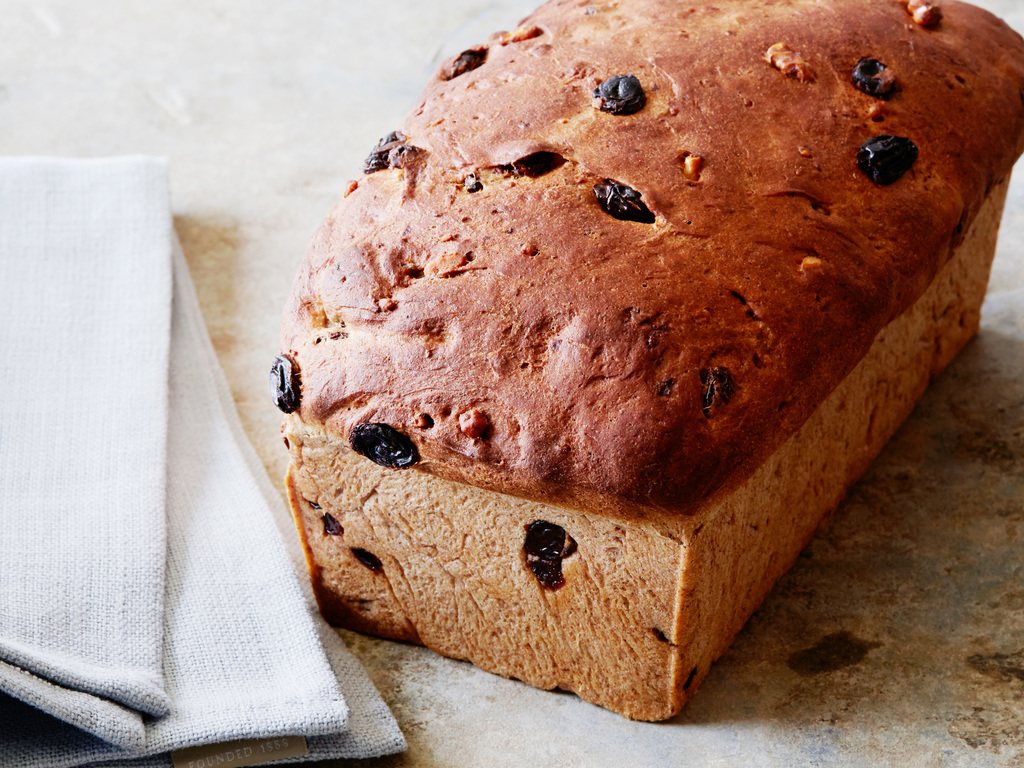
\includegraphics[width=\textwidth]{ch16_raisinbread.jpg}
	\end{center}
  \end{columns}
\end{frame}

\begin{frame}{Snakes on a @\#!\$\&\%*\&!*\$ Plane!}
  \begin{itemize}
	\item Imagine yourself a smooshed interstellar snake
	\item You live on a flat sheet of paper
	\item You can move around on the paper, but not up or down
	\begin{center}
	  \begin{tikzpicture}
		\draw[ultra thick, fill=LOrange] (0,0) --++(2,4) --++(3,0) --++(-2,-4) --cycle;
		\node[circle,rotate=0, xslant=.9, inner sep=0pt, outer sep=0pt] (sm) at (3,3) {\includegraphics[width=1cm]{ch26_snake.pdf}};
		\draw[thick, -latex, green] (sm.40)--+(40:.5);
		\draw[thick, -latex, green] (sm.-40)--+(-40:.5);
		\draw[thick, -latex, red] (.5,.5) --+(0,1);
		\draw[thick, -latex, red] (.5,0) --+(0,-.7);
	  \end{tikzpicture}
	\end{center}
	\item This is basically just the raisin loaf so far
  \end{itemize}
\end{frame}

\begin{frame}{Snakes on a Sphere}
  \begin{columns}
	\column{.5\textwidth}
	\begin{center}
	  \begin{tikzpicture}
		\fill[ball color=LOrange] (0,0) circle (2cm);
		\node[rotate=-120] at (-45:1.3) {\includegraphics[width=1cm]{ch26_snake.pdf}};
		\node[rotate=0] at (90:1) {\includegraphics[width=1cm]{ch26_snake.pdf}};
		\onslide<3>{
		  \fill[ball color=LOrange] (0,0) circle (3cm);
		  \node[rotate=-90] at (-45:2) {\includegraphics[width=1cm]{ch26_snake.pdf}};
		  \node[rotate=0] at (90:1.5) {\includegraphics[width=1cm]{ch26_snake.pdf}};
		}
	  \end{tikzpicture}
	\end{center}

	\column{.5\textwidth}
	\begin{itemize}
	  \item Suppose now we connected the ends of the paper to make it into a perfect sphere
	  \item Now your ```universe'' has:
		\begin{itemize}
		  \item No center
		  \item No edge!
		\end{itemize}
	  \item Looks the same regardless of where you are at
	  \item Cosmological principle \only<2->{\textcolor{green!70!black}{\LARGE\checkmark}}
	  \item Inflating the sphere will increase all the distances
	  \item The Hubble constant indicates how quickly the sphere inflates
	\end{itemize}
  \end{columns}
\end{frame}

\begin{frame}{Einstein's Demon}
  \begin{itemize}
	\item Einstein's General Relativity + a homogeneous universe predicts either an expansion or contraction of space
	\item Einstein hated this and was convinced it couldn't be true
	\item Originally added an extra term, a ``cosmological constant'' to his equations to allow for a static, unchanging universe
  \end{itemize}
  \begin{center}
	\begin{tikzpicture}
	  \node[inner sep=0pt, outer sep=0pt] at (0,0) {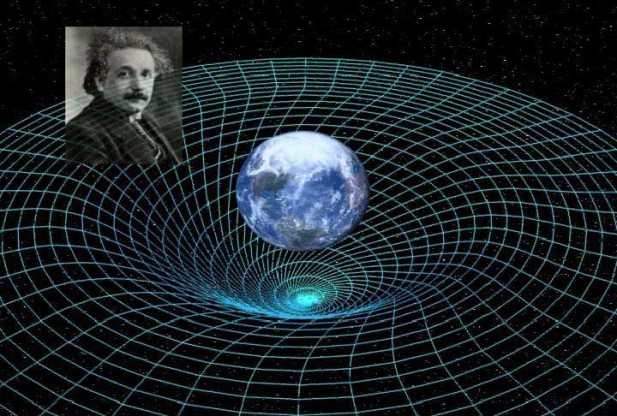
\includegraphics[width=6cm]{ch16_fieldeqns.jpg}};
	  \node[orange] at (6,0) {$\displaystyle R_{ab}-\frac{1}{2}Rg_{ab} = -8\pi T_{ab} + \Lambda g_{ab}$};
	\end{tikzpicture}
  \end{center}
\end{frame}

\begin{frame}{Einstein's Expanding Space}
  \begin{itemize}
	\item Galaxies appear to move only because space is expanding
	  \begin{itemize}
		\item Galaxies just conveniently mark points in space
	  \end{itemize}
	\item Space was expanding long before there were galaxies though
	\item Galaxies remain the same size
	  \begin{itemize}
		\item Gravity holds them together and determines the size
	  \end{itemize}
	\item Light is red-shifted because space expands so the wavelength is stretched
  \end{itemize}
  \begin{center}
	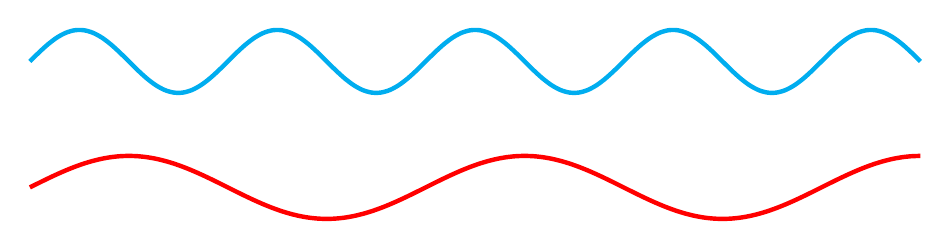
\begin{tikzpicture}[scale=.4]
	  \draw[cyan, domain=0:9*pi, smooth, samples=100, ultra thick] plot (\x, {sin(deg(\x))});
	  \draw[red, domain=0:9*pi, smooth, samples=100, ultra thick] plot (\x, {sin(deg(0.5*\x))-4});
	\end{tikzpicture}
  \end{center}
\end{frame}

\begin{frame}{Expansion and Age}
  \begin{itemize}
	\item If everything is expanding, we can reverse it to figure out how old the universe is
	\item ``Hubble Time''
	  \[t_h \approx \frac{1}{H}\]
	\item Comes out to about 14 billion years
	\item Or at least that's when the universe would have been a tiny point
	\item Note that this assumes the rate of expansion is constant!
  \end{itemize}
\end{frame}

\begin{frame}{Evidence of Billion-Year Timescales}
  \begin{center}
	\begin{tikzpicture}
		\clip (0,0) rectangle +(20cm,-6cm);
	  \node[inner sep=0pt, outer sep=0pt,anchor=north west] at (0,0) {\includegraphics[width=\textwidth]{ch16_deepfield.jpg}};
	  \node[draw, orange, fill=black, fill opacity=0.7, text opacity=1, rounded corners, align=center] at (12,-5.25) {Looking into space is\\ looking back in time};
	\end{tikzpicture}
  \end{center}
\end{frame}

\begin{frame}{The Hubble Xtreme Deepspace 3D!}
  \begin{center}
	\inlineMovie{../Videos/deepfield_fly.ogv}{../Videos/deepfield_fly.png}{width=.8\textwidth}
  \end{center}
\end{frame}

%\begin{frame}{A Trip Down Memory Lane}
  %\begin{center}
	%\includegraphics[width=.9\textwidth]{ch16_hubble_early_universe.jpg}
  %\end{center}
%\end{frame}

%\begin{frame}{Galaxy Evolution}
  %\begin{itemize}
	%\item Build up a sort of yearbook of galaxy ages
	  %\begin{itemize}
		%\item Looking at more distance objects means we are looking at younger objects
	  %\end{itemize}
	%\item Do we see a trend between spiral, elliptical and irregular galaxies over time?
	  %\begin{itemize}
		%\item Not really, they all follow their own path
	  %\end{itemize}
	%\item So why the different types?
  %\end{itemize}
%\end{frame}

%\begin{frame}{A Product of their Time}
  %\begin{itemize}
	%\item Two main ideas though to determine galaxy type:
	  %\begin{itemize}
		%\item \textcolor{Orange}{Initial rotation rate:} Perhaps with a small enough angular momentum, galactic disks never form and they stay elliptical
		%\item \textcolor{Orange}{Initial density:} Clouds with a high gas density would have formed stars much faster, and maybe used up all the gas before it had a chance to collapse into a disk
	  %\end{itemize}
	%\item Observations of a few massively redshift elliptical galaxies:
	  %\begin{itemize}
		%\item Lack blue and white stars
		%\item Even though universe still quite young
		%\item Supports fast star formation theory?
	  %\end{itemize}
	%\item Collisions and gravitational tugs likely played major roles in subsequent shaping
  %\end{itemize}
%\end{frame}

%\begin{frame}{A Slowing Expansion\ldots}
  %\begin{itemize}
	%\item We've been assuming that space expands at a constant rate
	%\item But gravity is attractive, and should be slowing that expansion?
	%\item Are we overestimating the lifetime of the universe?
  %\end{itemize}
%\end{frame}

\end{document}

